\chapter{Introduction}\label{cap.introduccion}
\setlength{\parindent}{0pt}
This work is focused in the problem of visual object tracking of multiple objects using deep learning and tracking-by-detection techniques. In this chapter, the context of this project is presented. Finally, the main objectives of this thesis and the methodology used to fulfil them are going to be explained.

\section{Multiple Object Tracking in Computer Vision}
The Multiple Object Tracking or \textit{MOT} is an important computer vision problem which continues to attract attention because of its potential in both the academic and commercial spheres. The real-world applications of the multiobject tracking are numerous including human-computer interaction, autonomous vehicles, robotics, video indexing, surveillance or security, among others. The computer vision community have been making big efforts in the past few decades to solve the MOT problem but the task is still open for improvement.\\ Many autonomous car projects are taking place globally which require solutions to various different problems including to keep an eye to all other moving objects in the area where the car is located (Figure \ref{fig:adas_tracking}). The outputs from the tracking module are a basic input for other modules like maneuver planning and trajectory planning. Autonomous vehicles are key in the continuous progress made in tracking and in the computer vision community in general. Many multi-object tracking algorithms have been proposed to solve the problem of real-world traffic monitoring. In these kind of tasks, the algorithms have to deal with complex occlusion situations and difficult object matching.\\
In an era where human-computer interaction has become particularly important, the hand is of big interest. Therefore, the object tracking is an important part of this area. For example, it is being used for tracking the hand movements because of its non-intrusive nature compared to other types of sensing which could imply the user to wear gloves, among others. With this tracking we can develop very interesting applications that range from predicting sign language to games like playing ``hand ping pong".
\\
 One of the most studied tracking areas is the pedestrian tracking, mainly because this particular kind of object can be seen in a large number of applications with commercial potential. As some studies indicate [1], about the 70\% of the current research done in MOT is dedicated to pedestrians. The difficulty of MOT lies in various challenging situations that can occur such as variation of the illumination, variation of scale, target deformation or fast motion. Most of this challenges are common to Single Object Tracking (\textit{SOT}) but MOT also needs to solve two main tasks: determining the number of objects and mantaining its identities over the time.\\
\begin{figure}[H]
\begin{center}
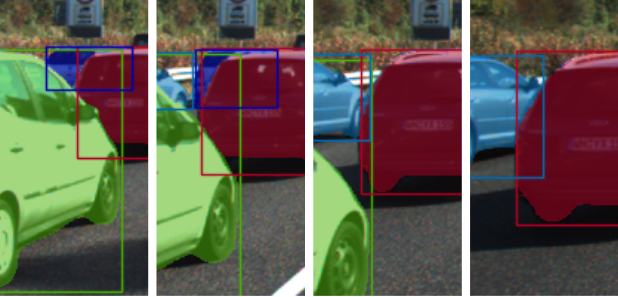
\includegraphics[scale=0.4]{figures/adas_tracking.png}
\caption{The importance of tracking in the autonomous vehicles \cite{voigtlaender2019mots}}
\label{fig:adas_tracking}
\end{center}
\end{figure}
\section{Deep Learning in Computer Vision}
Since the birth of Artificial Intelligence (AI) in 1956, the computer vision has followed a great rhythm of evolution. The AI has taking the machines to equal humans in the resolution of some tasks and, in certain cases, to overcome them.
Artificial intelligence is defined in~\cite{mccarthy2006proposal} as ``the subfield of Computer Science dedicated to developing programs that allow computers to present behaviors that can be characterized as intelligent". Machine learning (\textit{ML}) is defined in~\cite{samuel2000some} as ``a field of Computer Science that gives computers the ability to learn without being explicitly programmed". Therefore, given this definition, the ML can be considered a subfield of the AI.\\
One of the most well known and currently growing ML subfields is called \textit{Deep Learning}~\cite{deng2014deep}. This type of algorithm is intimately linked with the \textit{Artificial Neural Networks (ANNs)} and, in practice, they are usually used in an equivalent way although they are not the same. One of the aspects to be highlighted in the Deep Learning algorithms is that it is no longer necessary to extract feature vectors for the input to the machine learning system. This is because these algorithms ``learn" how to represent the data in a hierarchical way. From these networks, the \textit{convolutional neural networks (CNNs)} have a special interest to face the problem that this project presents. This type of networks are characterized by the use of a convolution operation in at least one of the layers of the network and they are designed for the processing of two-dimensional data such as images ~\cite{liu2015implementation}.\\
In the \textit{Artificial Intelligence} era the multi-object tracking makes use also from the AI to improve the tracking algorithms. These techniques are being used for a broad range of applications such as object detection, image classification, biometrics or medical imaging, among others (Figure \ref{fig:ssd_detection}). In most cases, the Deep Learning has beaten the previous State-of-the-Art in these areas.
\begin{figure}[H]
\begin{center}
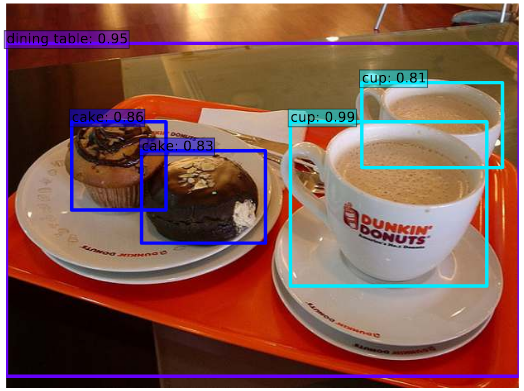
\includegraphics[scale=0.35]{figures/ssd_detection.png}
\caption{Object detection using deep learning techniques \cite{liu2016ssd}}
\label{fig:ssd_detection}
\end{center}
\end{figure}
A popular example of image classification is the case of classifying a handwritten digit (multiclass classification) from the MNIST dataset. Numerous applications can surge from recognizing digits and numbers like the automated recognition of house numbers in Google Street View images (Figure \ref{svhn}).
\begin{figure}[H]
\begin{center}
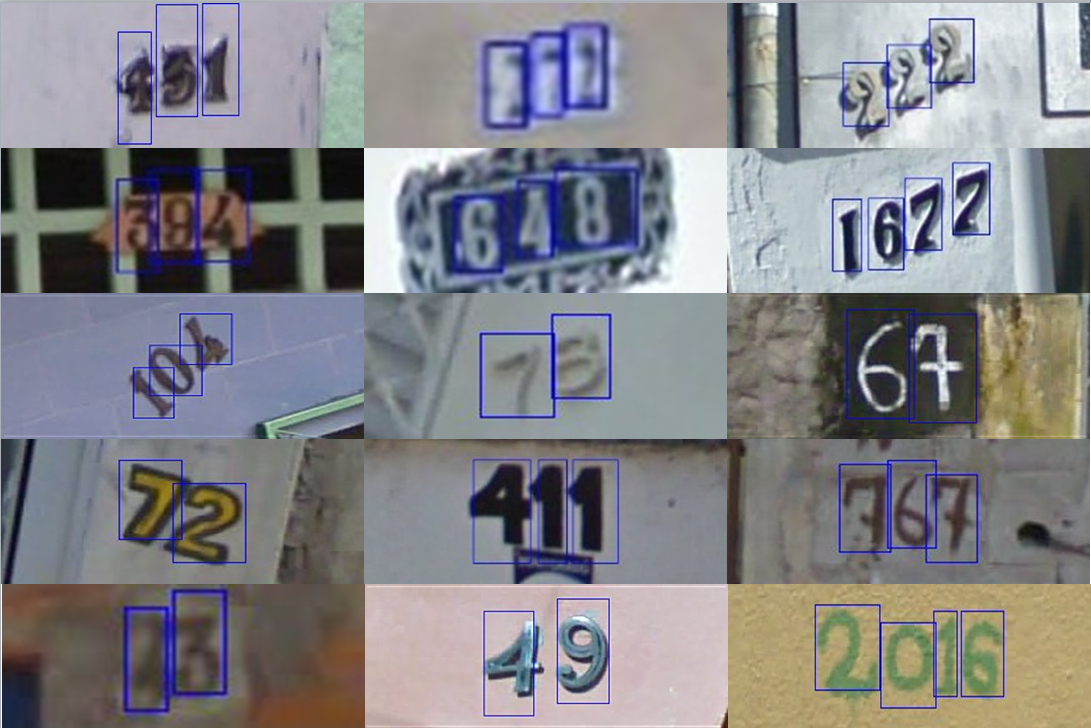
\includegraphics[scale=0.3]{figures/svhn.png}
\caption{Digit recognition on SVHN dataset \cite{netzer2011reading}}
\label{svhn}
\end{center}
\end{figure}
Apart from the typical deep learning applications, in the last few years other applications that can be tagged as ``artistic" have emerged like, for example, the style transfer. The \textit{neural style transfer} consists on learning the style from one or more images and applying that style to a new image. This can give some very interesting results as it can be seen in Figure \ref{style_transfer}. There are other examples of ``artistic" deep learning such as image colorization using deep learning. In this case, the neural colorization tries to convert a grayscale image to a color image which can be very helpful in areas like photography or the film industry.
\begin{figure}[H]
\begin{center}
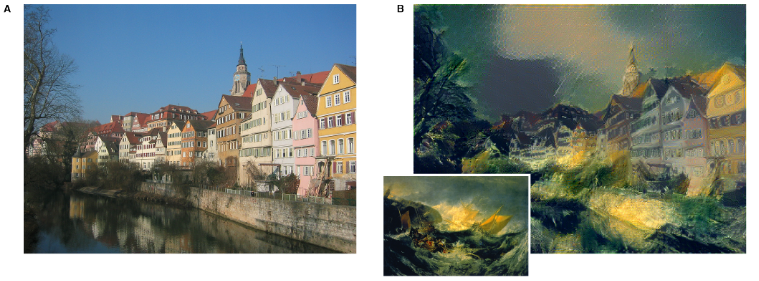
\includegraphics[scale=0.4]{figures/style_transfer.png}
\caption{Example of neural style transfer from famous artworks to a photograph \cite{gatys2015neural}}
\label{style_transfer}
\end{center}
\end{figure}
Given the broad areas of application where deep learning is succeeding and the ones who are still in research it is going to be studied on this master thesis the use of deep learning techniques to tackle the multi-object tracking problem.\\
The deep learning for tracking has been used in previous works from other colleagues such as Marcos \cite{tfm-marcos}. In his work, the task is a visual tracking on people using deep learning with a classical feature tracking based on the Lucas-Kanade algorithm \cite{baker2004lucas}. The detections obtained by the neural networks allow to build a robust hybrid tracker. However, these detections are calculated in an offline way before launching the tracking.\\
Other interesting works with neural networks, in this case, for object detection have been developed such as \textit{Object Detector} \cite{condes2018person}.
This application is composed of three modules working as three  asynchronous threads. These modules are: a \textit{Camera} that provides the images, a \textit{GUI} that provides the user interface and a \textit{DetectionNetwork} that encapsulates an object detector neural network. As a result this node allows the user to visualize object detections, i.e.\ bounding boxes drawn over the image in real-time. The images can be obtained from different sources as a webcam, a video or via remote proxy. It also provides functionality to perform on-demand detection. The Figure \ref{fig:object_detector} shows the Object Detector running.
\begin{figure}[H]
\begin{center}
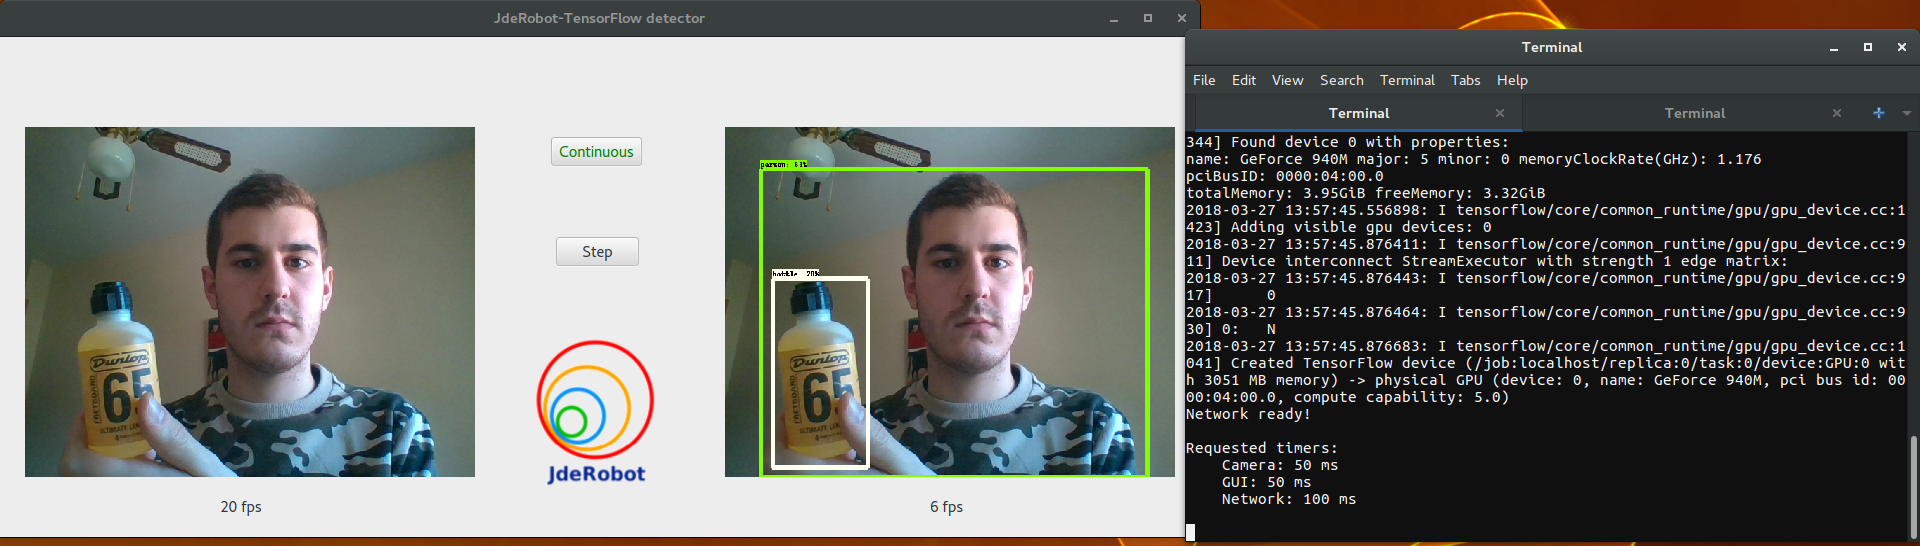
\includegraphics[scale=0.25]{figures/object_detector.png}
\caption{Example of the Object Detector node working in real-time (from \href{https://github.com/JdeRobot/dl-objectdetector}{Object Detector official repository})}
\label{fig:object_detector}
\end{center}
\end{figure}
The user can download pre-trained open neural network models for \textit{Tensorflow} or \textit{Keras} and configure the Object Detector to work with them.\\
As it has been seen, the deep learning and the multiobject tracking are still open areas where multiple applications can be obtained.\\
\section{Objectives}
The main objective of this master thesis is to build a multi-object tracking application which makes use of two techniques: deep learning and 2D-tracking. In this work we are going to study how to use the best of both techniques to build a robust and fast multiobject tracker which can be capable of run in resource constrained hardware on real-time. This work takes the form of a user application and allows multiple configurations. The developed solution will be tested with well-known datasets of multiobject tracking challenges which will provide the performances obtained by each configuration of the application and finally, it will allow the selection of the best configuration.\\
This task can be divided into different subobjectives:
\begin{enumerate}
\item \textbf{Development of an object detector using deep learning}\\\label{first_objective}
Learn the fundamentals of object detection using deep learning techniques. Study the performance on both accuracy and speed of these techniques in datasets. Finally, select the default object detector.
\item \textbf{Development of a visual tracking module}\\
Build the tracking module taking into account the necessity of speed in constrained resources.
\item \textbf{Combination of neural object detection and object tracking in a single software component}\\
Integration of the modules needed into a thread infrastructure. This will imply a sophisticaded synchronization between them.
\item \textbf{Experimental validation}\\
Finally, several experiments with state-of-the-art datasets will be performed to validate the developed solution and select the best configuration based on the extracted results.
\end{enumerate}

\section{Methodology} \label{Methodology}
The following tools have been employed to follow the project progress and making it visible for the community:
\begin{itemize}
    \item \textbf{GitHub repository:} the code of the project is publicly available on GitHub and was constantly updated. The repository can be accessed in the link\footnote{ \url{https://github.com/RoboticsURJC-students/2017-tfm-alexandre-rodriguez}}.
    \item \textbf{Wiki:} it has been used as a blog of the progress of the project. In the link\footnote{ \url{http://jderobot.org/Arodriguez-tfm}}, the steps followed to achieve this target can be seen.
\end{itemize}
The development of this project has been weekly followed by the tutor. In this weekly meetings the work done in the previous week was evaluated and discussed ending in new milestones for the following week. This continuous feedback allowed a better development of the project both in terms of understanding the topic in question and also in terms of time management.\\

